\section{Accessibilità}
\subsection{Colori}
La gamma cromatica utilizzata nel sito web sviluppato è stata ristretta in modo tale da garantire un buon contrasto tra contesto e testo. Per arrivare alle nostre conclusioni per quanto riguarda i colori ci siamo
serviti di un estensione per Google Chrome, \textit{Colorblindly}. Ci ha permesso di testare il nostro sito con i quattro tipi di daltonismo più diffusi: protanopia, deuteranopia, tritanopia e acromatopsia. In questo modo, il sito risulta accessibile a tutte le categorie di utenti con difficoltà visive.\\
Dove possibile, inoltre, si adottano colori definiti \textit{web safe}\footnote{\url{https://www.color-hex.com/216-web-safe-colors/}}, in modo tale da garantire una corretta visualizzazione del sito su un maggior numero di dispositivi.\\
Per verificare l'adeguatezza del contrasto dei colori usati per il testo ci siamo serviti dello strumento \textit{Colour Contrast Analyser}. Con quest'ultimo è stato possibile verificare che ogni abbinamento tra colore di sfono e colore del testo rispestasse un rapporto di contrasto tale da essere conforme con i seguenti criteri:
\begin{itemize}
	\item 1.4.3 Contrast (Minimum)
	\item 1.4.6 Contrast (Enhanced)
	\item 1.4.11 Non-text Contrast
\end{itemize} 
presenti nelle linee guida WCAG 2.1.\footnote{\url{https://www.w3.org/TR/WCAG21/}} 

\subsection{Immagini}
Le immagini all'interno del sito sono tutte accompagnate dall'attributo \textit{alt} al quale è stata assegnata una descrizione esaustiva dell'immagine. Ciò rende le immagini accessibili anche alle categorie di utenti con difetti visivi, poiché lo screen-reader si avvarrà di tali descrizioni.

\subsection{Scelte progettuali}
In corso d'opera abbiamo fatto delle modifiche per raggiungere il più alto livello di accessibilità possibile.
Per rappresentare i dati tecnici delle auto esposte subito avevamo optato per la rappresentazione in forma
tabellare, ma ci siamo presto resi conto che poteva essere un ostacolo per uno screen-reader, quindi abbiamo
scelto la rappresentazione attraverso elenco. \\
La navbar nativamente era di colore giallo come il logo, ma dopo alcuni test ci siamo resi conto che non era
la scelta ideale per un utente con problemi di acromatopsia, quindi abbiamo usato il grigio e il nero. \\
Avevamo dato per scontato che mettendo la mappa del luogo del museo fosse chiaro dove recarsi, ma non avevamo
pensato che uno screen-reader avrebbe potuto aver problemi nell'interpretarla correttamente, è stato quindi aggiunto all'interno della pagina in questione l'indicazione testuale dell'indirizzo del museo.


\subsection{Navigazione nel sito}
La navigazione nel sito è garantita, in primo luogo, da una semplice \textit{navbar} che non include sottomenù, come illustrato in §\ref{design}. Sono direttamente visibili e accessibili tutte le pagine del sito web:
\begin{figure}[h]
		\begin{center}
		
\includegraphics[scale=1.312]{Images/headerSito.png}
		\caption{Header del sito, in particolare visto dalla pagina mostre.}
	\end{center}
\end{figure}\\
Inoltre, il posizionamento corrente all'interno del sito web è chiarito grazie all'evidenziazione della pagina corrente all'interno della navbar:
\begin{figure}[h]
	\begin{center}
		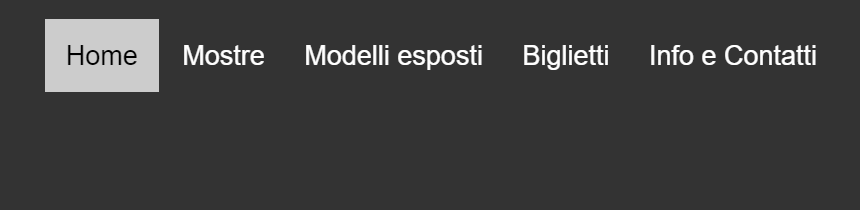
\includegraphics[scale=1.312]{Images/selezionePaginaCorrente.png}
		\caption{Dettaglio: la pagina corrente è evidenziata rispetto alle altre.}
	\end{center}
\end{figure}\\
Oltre a ciò, sotto l'intestazione del sito è presente l'indicazione testuale sulla corrente posizione all'interno del sito ("\textit{breadcrumbs}"):
\begin{figure}[h]
	\begin{center}
		
\includegraphics[scale=0.6]{Images/breadcrumbs.png}
		\caption{Dettaglio: \textit{breadcrumbs}.}
	\end{center}
\end{figure}\\
Per quanto concerne i link presenti nel sito, è stato fatto in modo che link "\textit{visitati}" e "ancora da visitare" siano facilmente distinguibili. Un esempio è visibile di seguito.
\begin{figure}[h]
	\begin{center}
		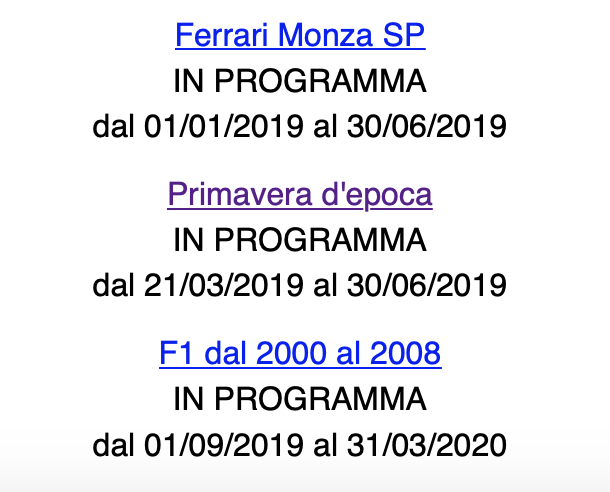
\includegraphics[scale=1.5]{Images/linkVisitatiDaVisitare.png}
		\caption{Dettaglio: link da visitare e visitati. Il link centrale è stato già visitato mentre il primo e l'ultimo risultano ancora da esplorare.}
	\end{center}
\end{figure}

Per rendere efficiente la navigazione all'interno del sito anche ad utenti con difficoltà visive, è stato fatto uso di \textit{tabindex} per consentire un'agile navigazione all'interno del sito. Ogni immagine è inoltre accompagnata da un \textit{alt} che descrive in modo soddisfacente l'immagine in oggetto.\\
È stato deciso di non introdurre \textit{accesskey} poiché gli shortcut stabiliti avrebbero potuto entrare in conflitto con i comandi definiti di default dai browser.\\
È stato inoltre inserito un bottone che consente di tornare facilmente in testa alla pagina.

\subsection{Mobile}
Per cercare di rendere il sito compatibile con la maggior parte dei dispositivi mobile (Smartphone, tablet...)
abbiamo deciso di implementare l'accessibilità con CSS puro.
\\ ...

\subsection{Test accessibilità}
Con lo scopo di verificare e accertarsi che i livelli di accessibilità raggiunti fossero soddisfacenti sono stati effettuati dei test. Tali test non hanno il presupposto di essere esaustivi, ma piuttosto informativi.\\
Nei prossimi paragrafi mostriamo, con l'ausilio di alcuni screenshot, i risultati ottenuti.\\
...
\subsubsection{Test daltonismo}
Riportiamo di seguito i test effettuati sulla home page del sito per quanto riguardano i difetti visivi relativi alla cecità completa o parziale ai colori, noti come daltonismo.
\begin{figure}[H]
	\begin{center}
		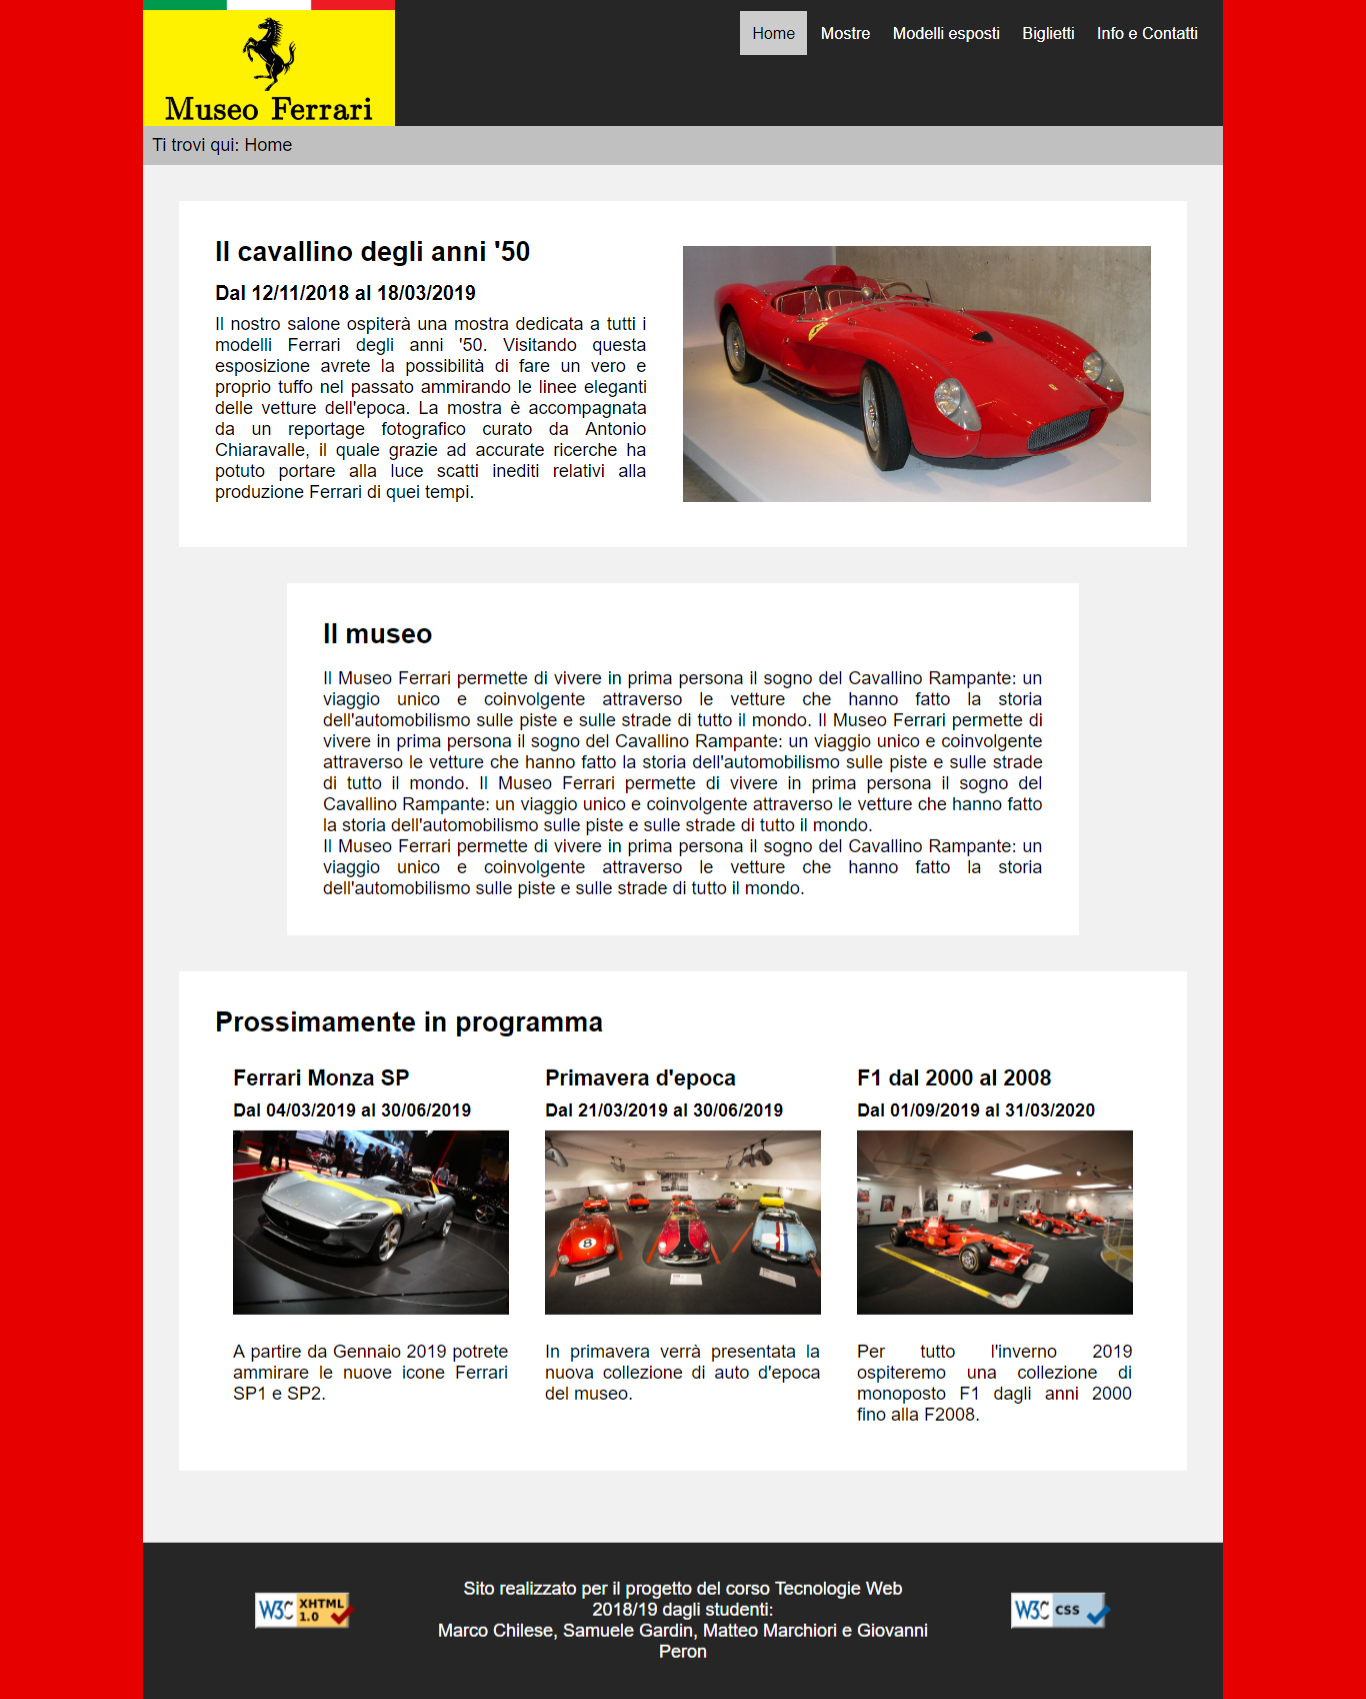
\includegraphics[scale=0.15]{Images/original.png}
		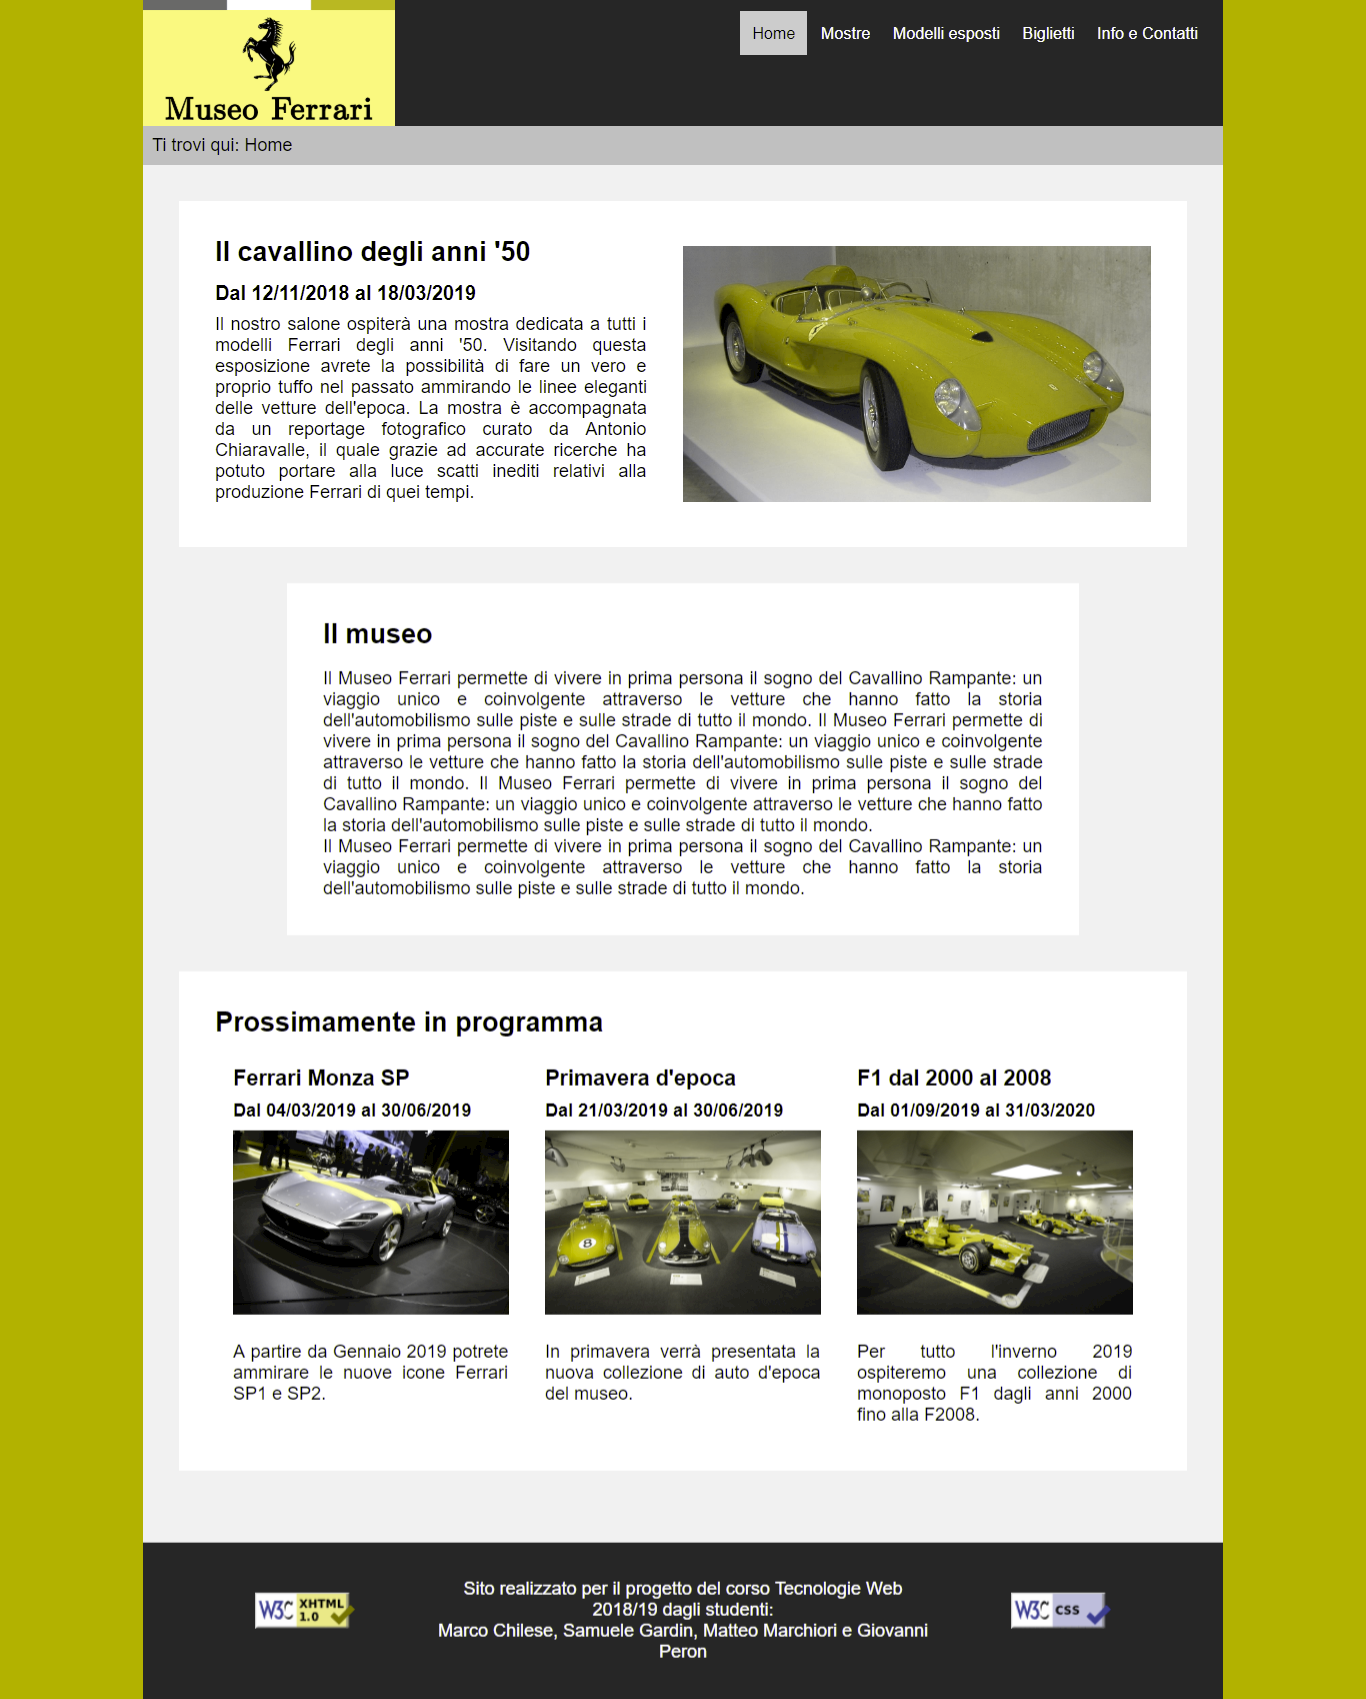
\includegraphics[scale=0.15]{Images/protanopia.png}
		\caption{Test daltonismo protanopia}
	\end{center}
\end{figure}

\begin{figure}[H]
	\begin{center}
		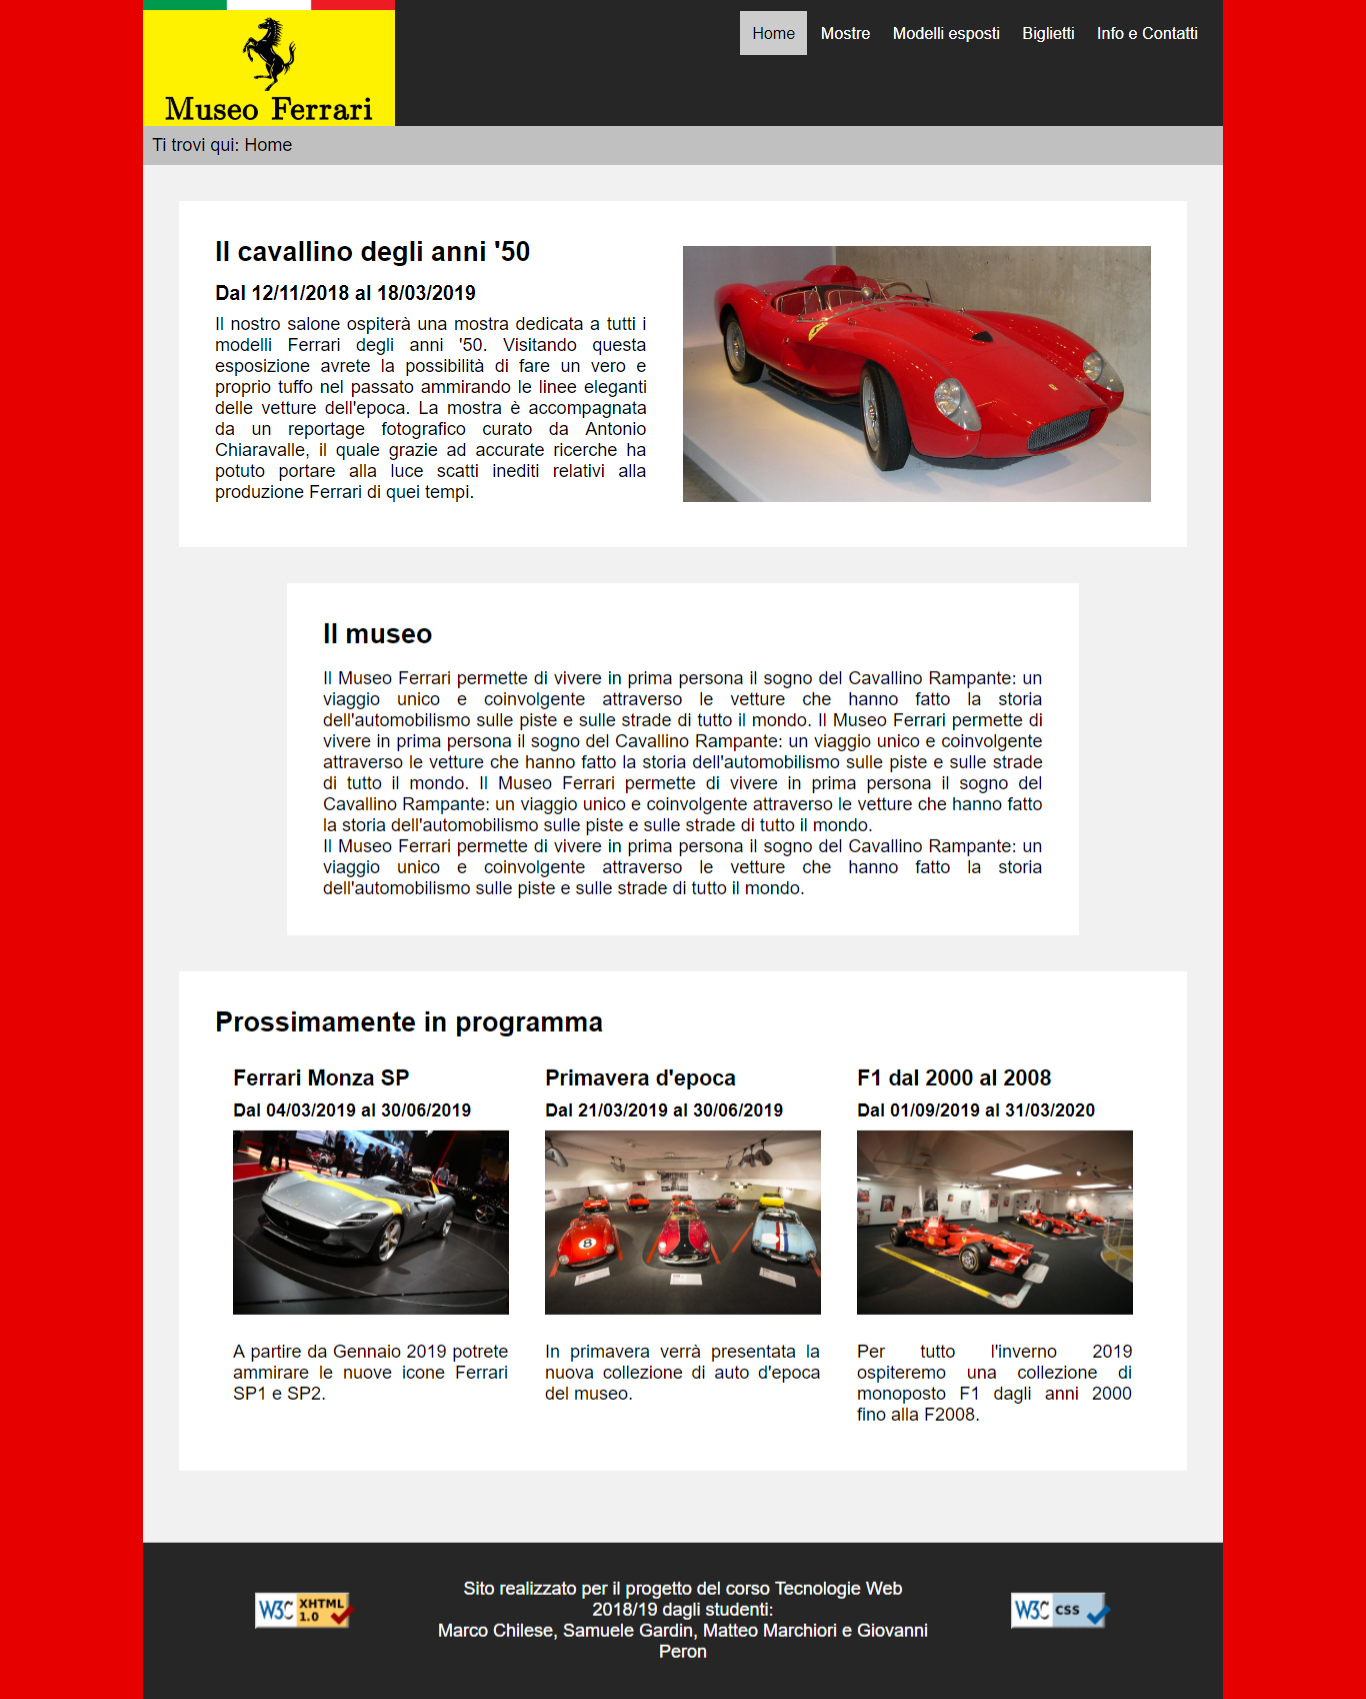
\includegraphics[scale=0.15]{Images/original.png}
		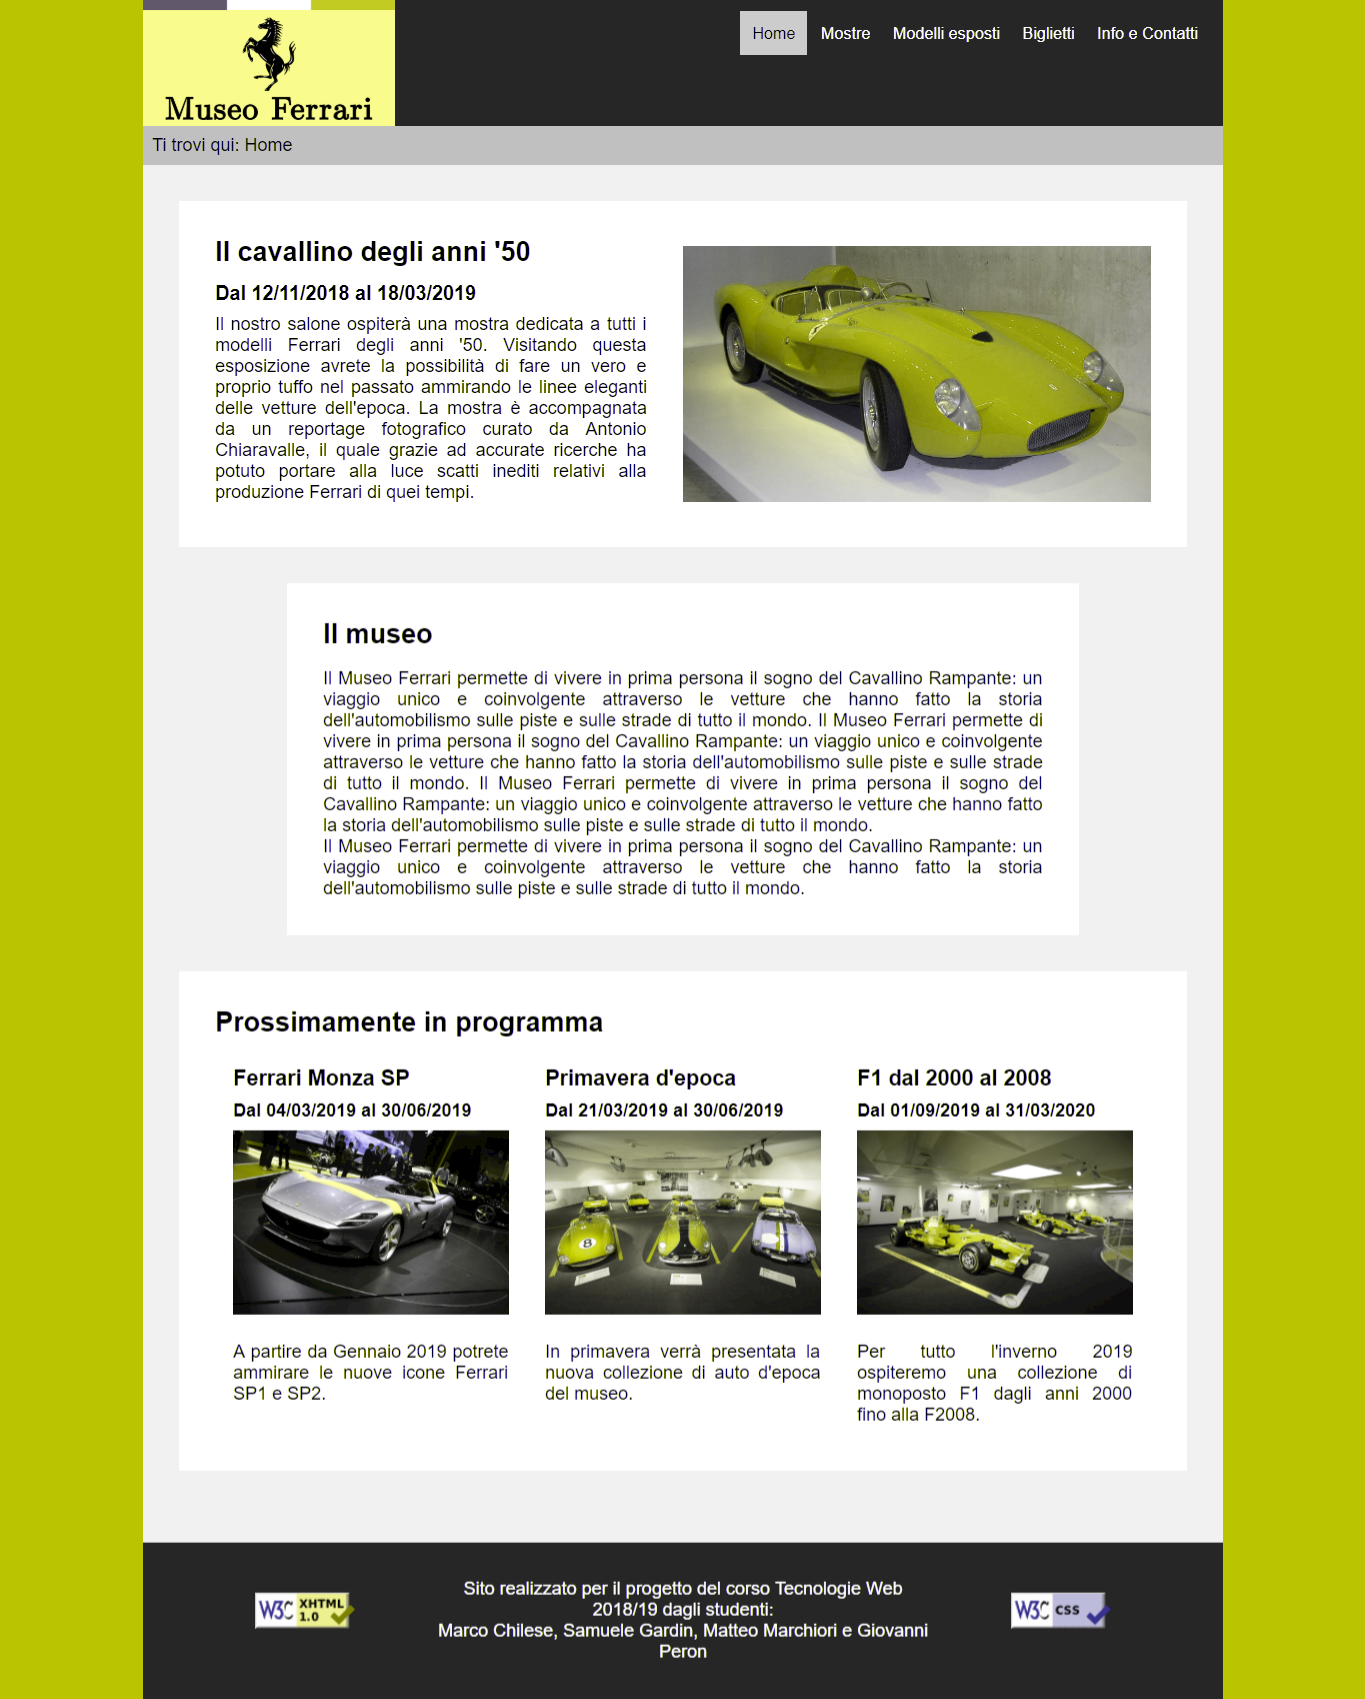
\includegraphics[scale=0.15]{Images/deuteranopia.png}
		\caption{Test daltonismo deuteranopia}
	\end{center}
\end{figure}

\begin{figure}[h!]
	\begin{center}
		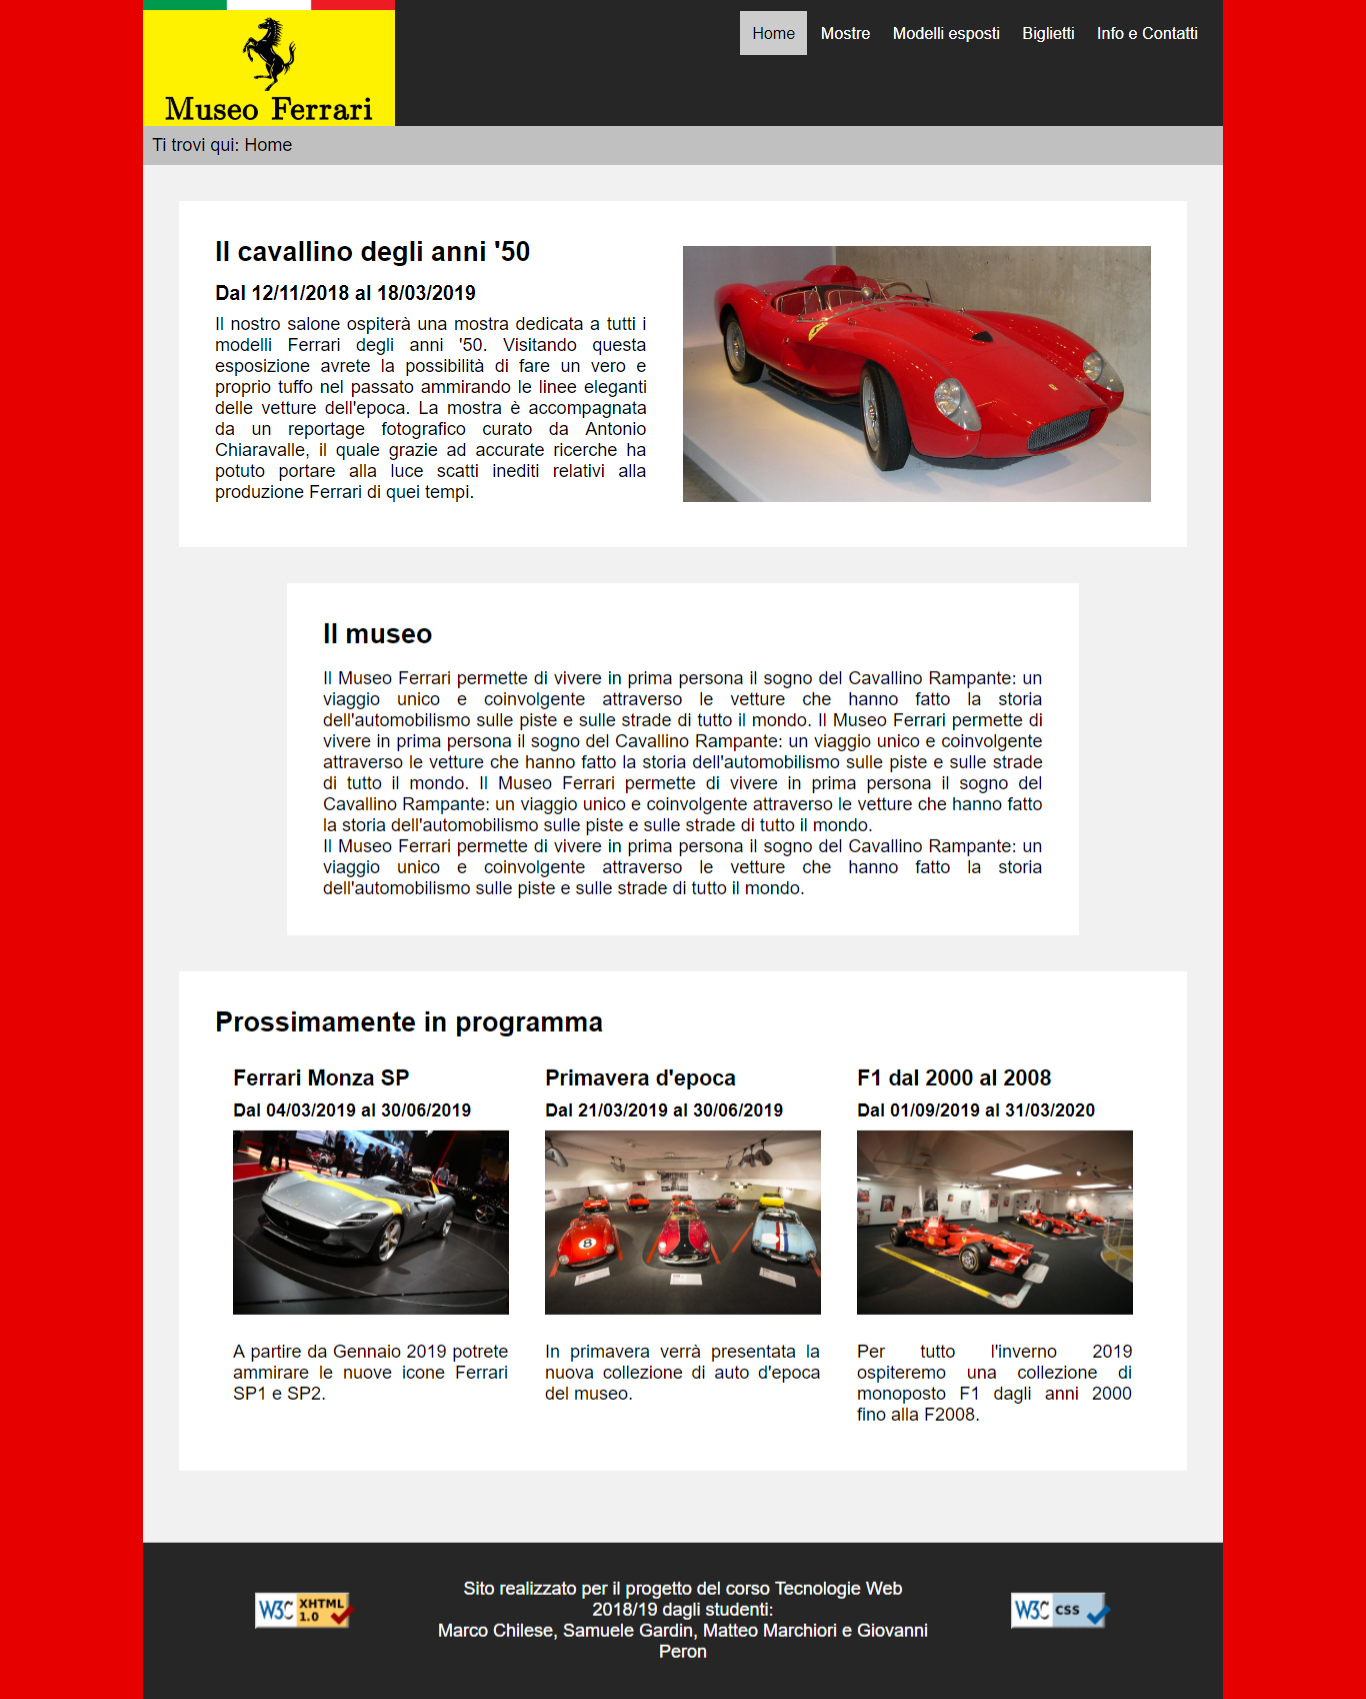
\includegraphics[scale=0.15]{Images/original.png}
		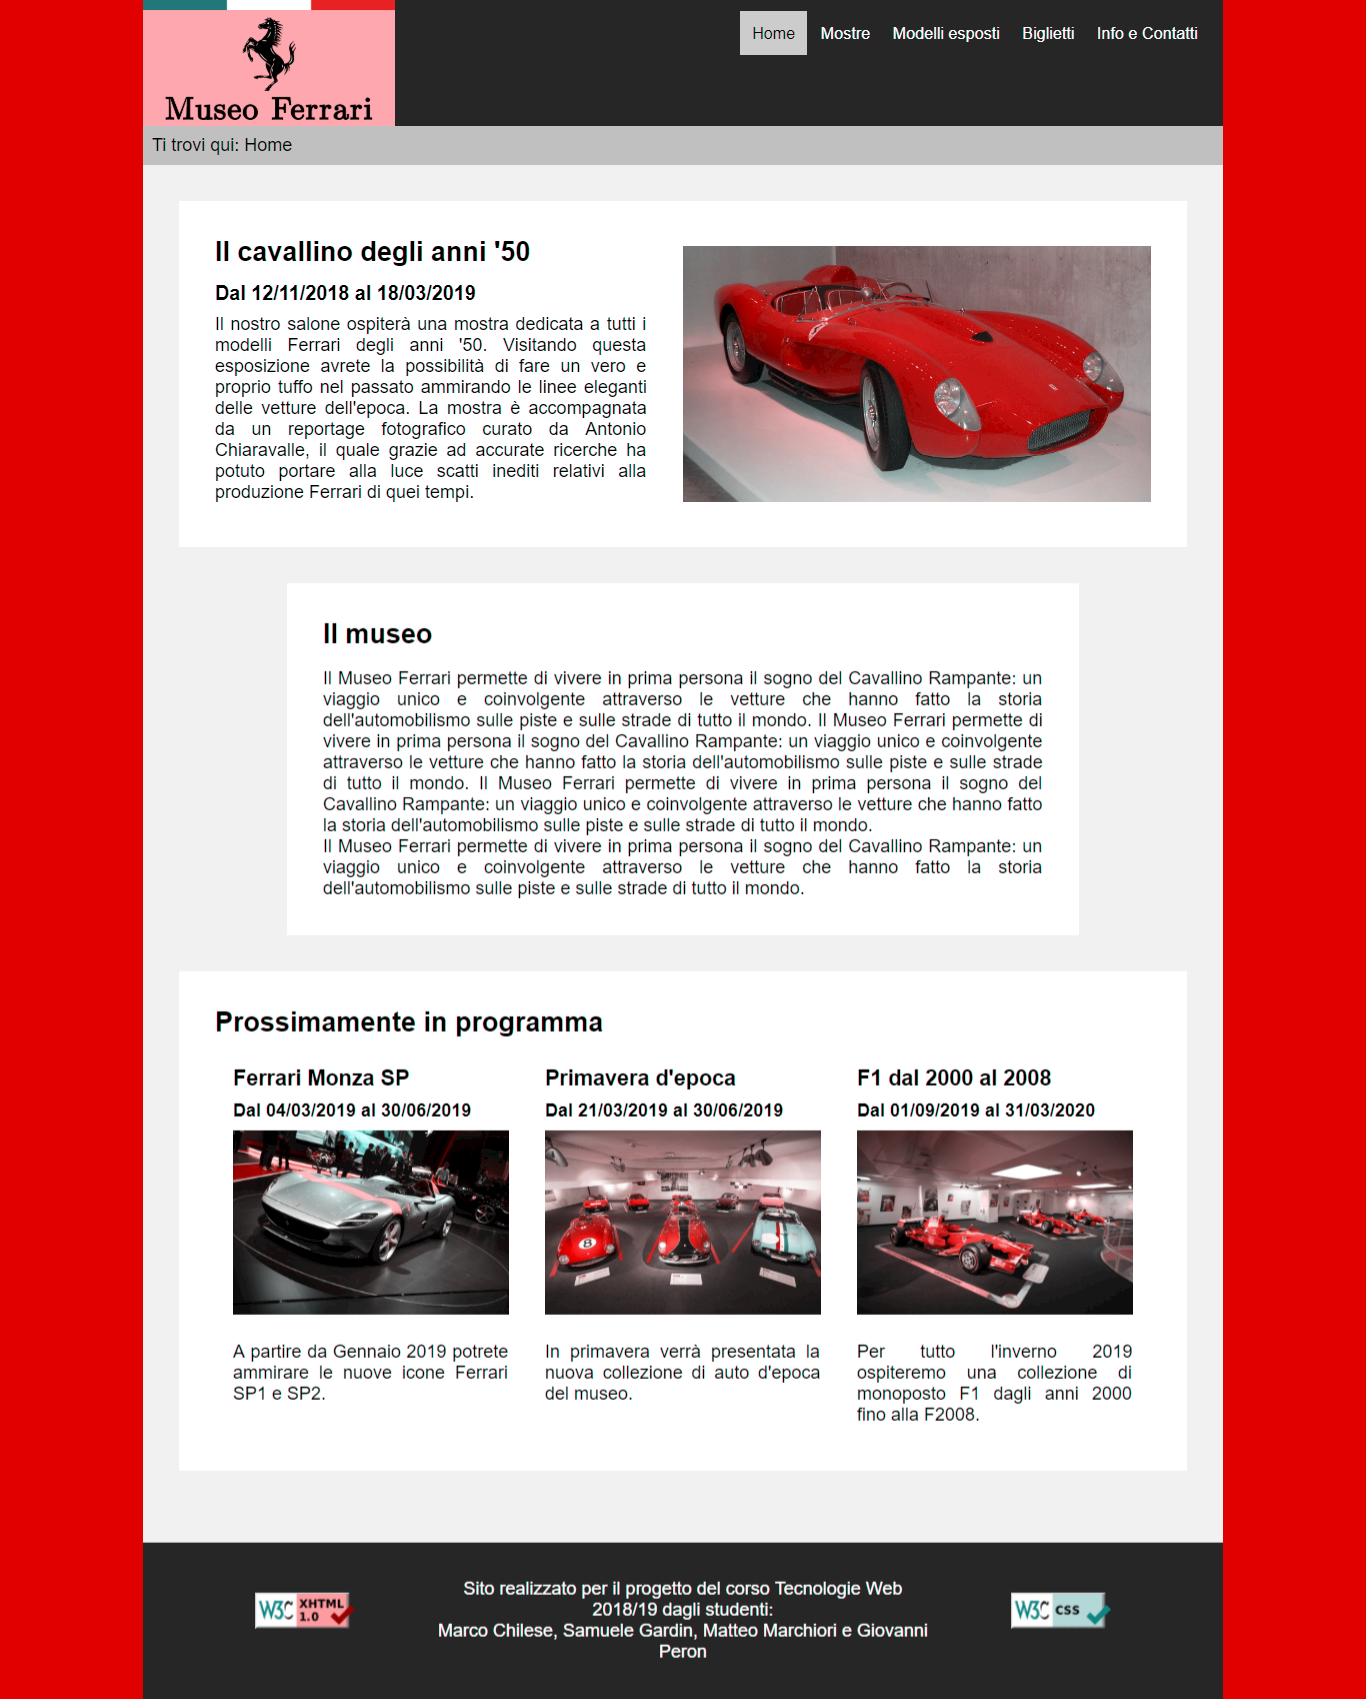
\includegraphics[scale=0.15]{Images/tritanopia.png}
		\caption{Test daltonismo tritanopia}
	\end{center}
\end{figure}

\begin{figure}[h!]
	\begin{center}
		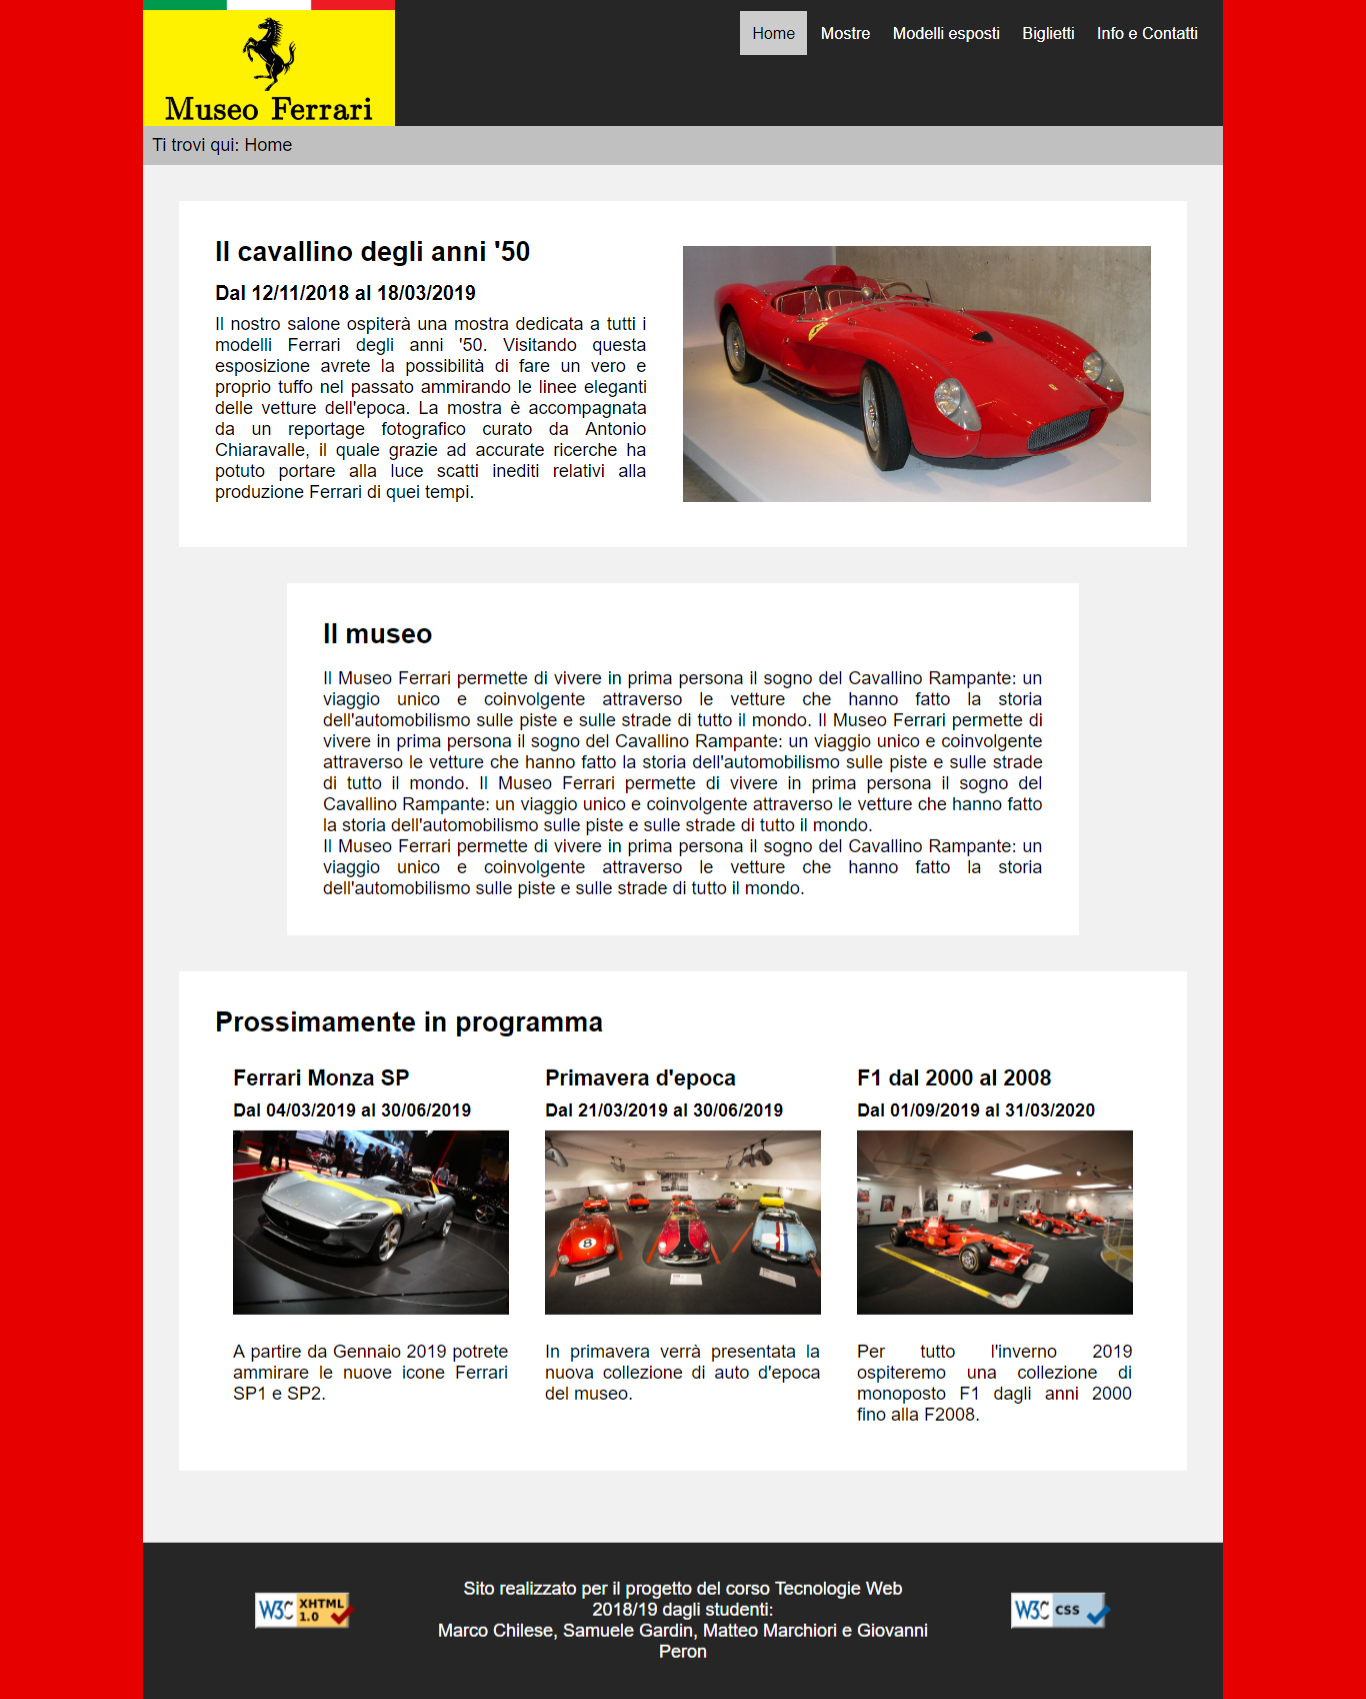
\includegraphics[scale=0.144]{Images/original.png}
		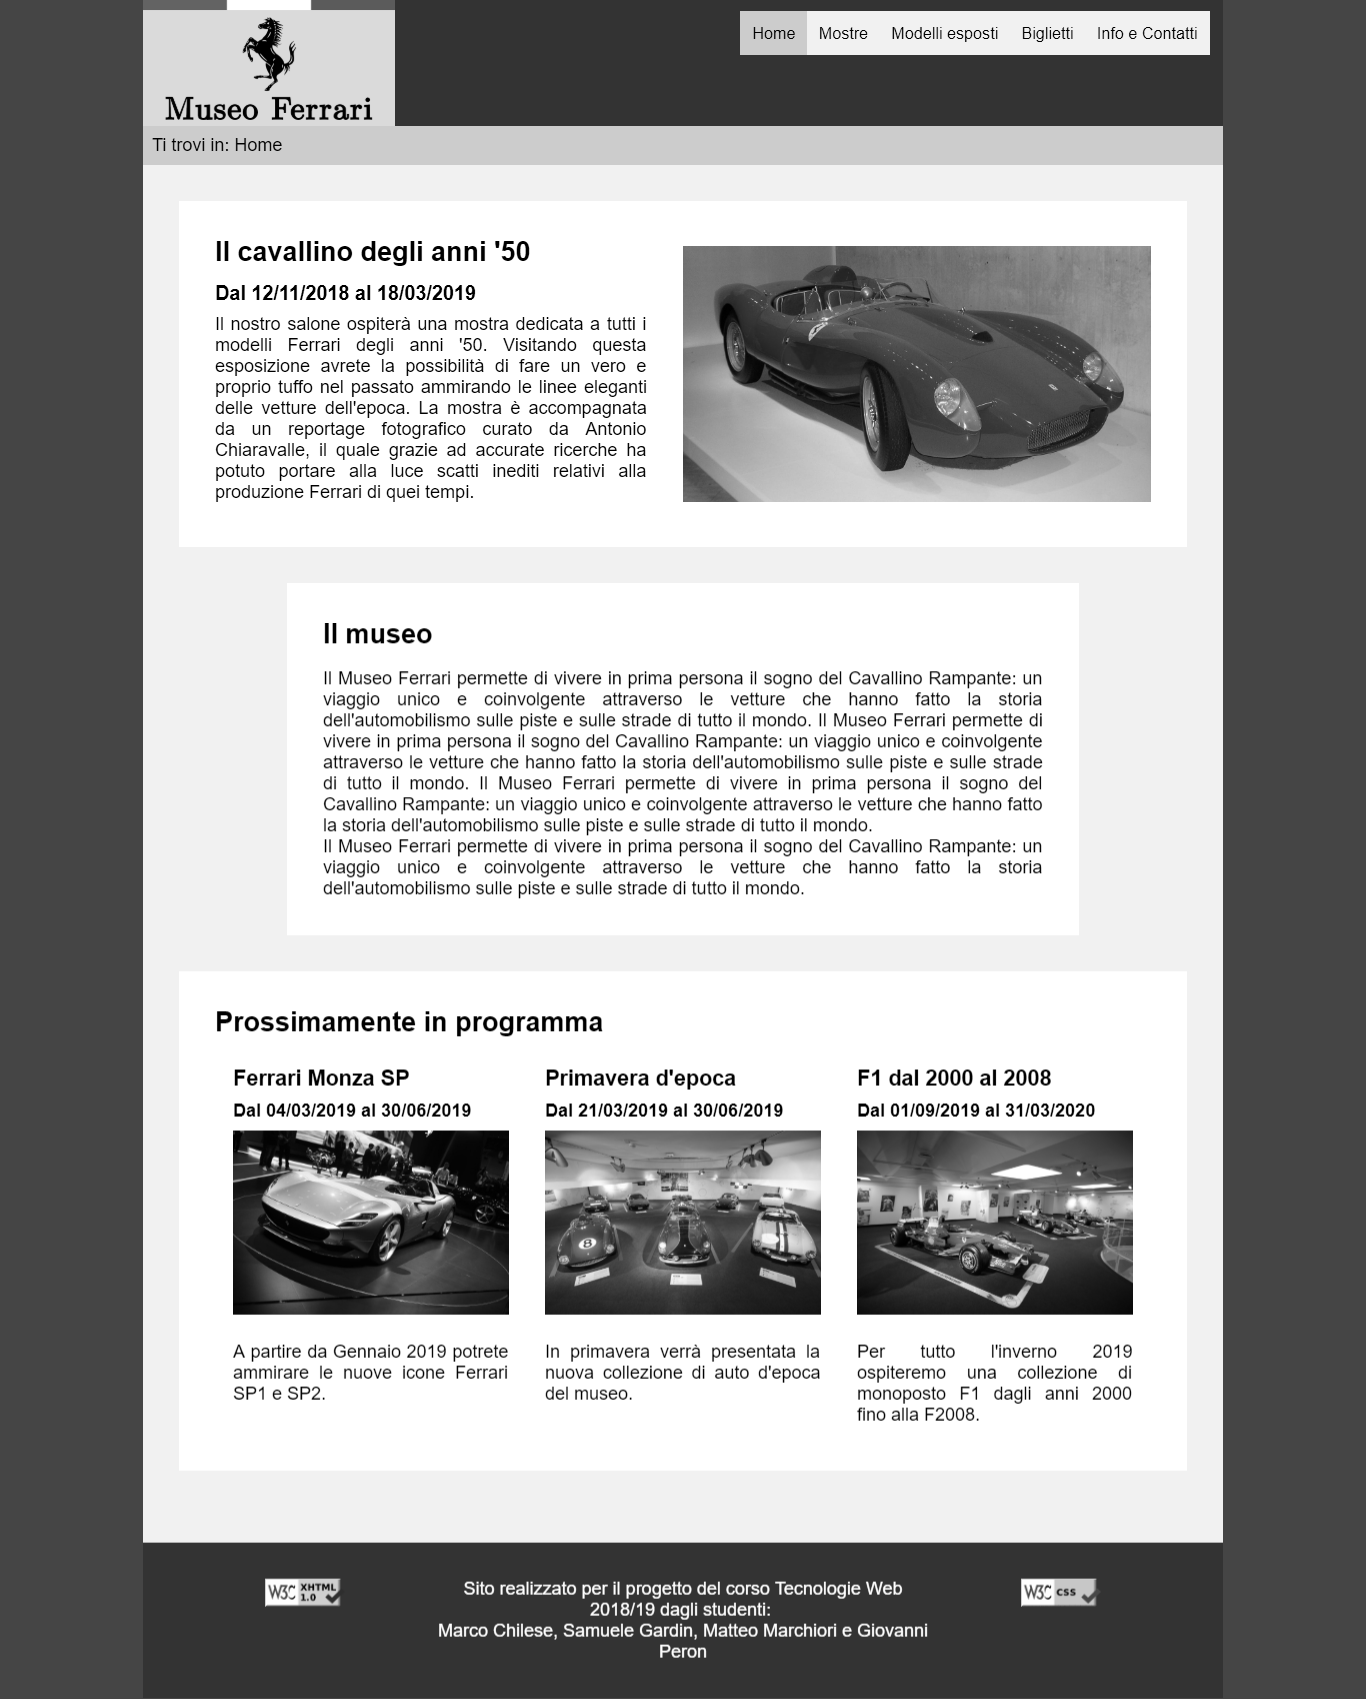
\includegraphics[scale=0.144]{Images/acromatopsia.png}
		\caption{Test daltonismo acromatopsia}
	\end{center}
\end{figure}

\subsubsection{Contrasto colori}
La seguente tabella espone i risultati ottenuti con lo strumento \textit{Colour Contrast Analyser} relativi ad ogni abbinamento tra colore di sfondo e colore del testo presente nel sito. Tutte le coppie di colori scelti rispettano i criteri 1.4.3 Contrast (Minimum), 1.4.6 Contrast (Enhanced) e 1.4.11 Non-text Contrast, presenti nelle linee guida WCAG 2.1.

\newcolumntype{C}[1]{>{\centering\arraybackslash}p{#1}}

{\renewcommand{\arraystretch}{1.5}%
	\begin{longtable}[c]{|C{.14\textwidth}|C{.14\textwidth}|C{.13\textwidth}|m{.45\textwidth}|}
		\hline
		\rowcolor[HTML]{F1F1F1} 
		\textbf{Colore di sfondo} & \textbf{Colore del testo} & \textbf{Contrast ratio} & \multicolumn{1}{c}{\cellcolor[HTML]{F1F1F1}\textbf{Utilizzo nel sito}}\\ 
		\endhead
		\hline
		\#333333& \#FFFFFF & 12.6 : 1 & Simbolo hamburger del menù di navigazione, footer, label o legend, pulsanti\\ 
		\hline
		\#CCCCCC & \#000000 & 13.1 : 1 & Pagina corrente nel menù di navigazione, form delle pagine biglietti e info e contatti \\ 
		\hline
		\#F1F1F1 & \#000000 & 18.6 : 1 & Pagine non visitate nel menù di navigazione\\ 
		\hline
		\#F1F1F1 & \begin{tabular}[c]{@{}c@{}}\#800080 \\ (purple)\end{tabular} & 8.3 : 1  & Pagine visitate nel menù di navigazione\\ 
		\hline
		\#FFFFFF & \#000000  & 21 : 1 & Testo delle pagine del sito\\ 
		\hline
		\#FFFFFF & \begin{tabular}[c]{@{}c@{}}\#0000FF \\ (blue)\end{tabular} & 8.6 : 1 & Link non visitati nel sito ad esempio nella pagina mostre\\ 
		\hline
		\#FFFFFF & \begin{tabular}[c]{@{}c@{}}\#800080 \\ (purlpe)\end{tabular} & 9.4 : 1 & Link visitati nel sito ad esempio nella pagina mostre\\ 
		\hline 
		\#CCCCCC & \#990000 & 5.6 : 1 & Messaggi d'errore nei form\\ 
		\hline  
		\#CCCCCC & \#006600  & 4.5 : 1  & Messaggio stato di invio nel form biglietti\\ 
		\hline
	\end{longtable}
}
